\documentclass[a4paper,12pt]{article} % Tipo de documento y tamaño de letra.
\usepackage[utf8]{inputenc} % Para que reconozca caracteres especiales como tildes.
\usepackage[spanish]{babel} % Para definir el idioma y el formato de fechas en español.
\usepackage{amsmath, amssymb} % Paquetes para símbolos y ecuaciones avanzadas (Para hacer una ecuación con un recuadro).
\usepackage{ragged2e} % Para justificar textos.
\usepackage{multicol} % Para crear columnas.
\usepackage{slashed} % Para generar números o variables canceladas (Una línea diagonal sobre el número o variable)
\usepackage{graphicx} % Paquete para poner graficas.
\usepackage{float} % Para poder dejar la imagen en un punto fijo del documento.
\usepackage{longtable} % Para tablas largas.
\usepackage{cancel} % Para hacer cancelaciones en medio de operaciones.
\usepackage{xcolor} % Para el color y esas cosas.
\usepackage{apacite} % Paquete para citas APA.
\usepackage{fancyhdr} % Para personalizar encabezados y pies de página.
\usepackage{geometry} % Para ajustar márgenes.
\usepackage{setspace} % Para ajustar el interlineado.
\usepackage{natbib}  % Para manejar las citas y que no queden pegadas y feas :P.
\usepackage{hyperref} % Para que los enlaces sean clickeables.


\pagestyle{fancy}
\fancyhf{} % Limpia encabezados y pies de página predeterminados
\fancyhead[L]{\textbf{DINÁMICA, SÓLIDO RÍGIDO Y M.A.S.}} % Encabezado izquierdo
\fancyhead[R]{\textbf{FÍSICA ll}} % Encabezado derecho
\fancyfoot[C]{\thepage} % Número de página en el centro del pie

\geometry{headheight=12.96115pt, top=1in, bottom=1in, left=1in, right=1in}
\begin{document}


\begin{figure}[H] 
    \centering
    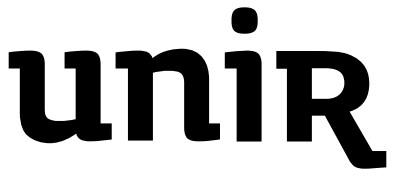
\includegraphics[width=0.5\textwidth]{Unir.jpg} 
\end{figure}

\vspace{\baselineskip}

% Ajustamos manualmente todo ;)
\begin{center}
    \textbf{\Large RESOLUCIÓN DE PROBLEMAS SOBRE MOMENTOS DE INERCIA Y FLUIDOS. } \\[0.3cm]
    \vspace{\baselineskip}
    \textbf{Liz Ángel Núñez Torres.} \\[0.4cm]
    \textbf{Grado en Física.} \\[0.4cm]
    \textbf{Universidad Internacional de La Rioja.} \\[0.4cm]
    \textbf{21 de marzo de 2025.}
\end{center}

\newpage
\tableofcontents
\newpage

\section{Ejercicio.}

\begin{figure}[H]
    \centering
    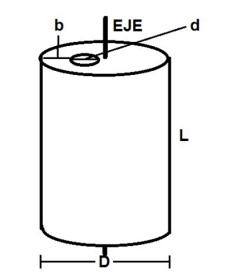
\includegraphics[width=0.3 \textwidth]{ejercicio1.jpg}
    \caption{Cilindro - Ejercicio 1.}
\end{figure}

\begin{justify}
    Calcula el momento de inercia de un cilindro de diámetro \(D\), altura \(L\) y
    densidad \(\rho\), que tiene, a una distancia \(b\) del borde, un agujero cilíndrico de diámetro \(d\), tal y como
    se puede ver en la Figura 1.
\end{justify}
\begin{justify}
    El agujero se encuentra a través de un eje que pasa por el centro del
    cilindro grande y es perpendicular a las caras circulares.
\end{justify}
\begin{itemize}
    \item La distancia \(b\) va desde el borde del cilindro de diámetro \(D\) hasta el borde exterior del
    cilindro de diámetro \(d\)
    \item El resultado debería expresarse en función de la densidad de la figura.
\end{itemize}

\subsection{Solución.}


\vspace{\baselineskip}

\textbf{Datos:}

\vspace{\baselineskip}


\textbf{Cilindro.}
\begin{itemize}
    \item Diámetro \( \Rightarrow D.\)
    \item Radio \(R \Rightarrow \frac{D}{2}\).
    \item Altura \(\Rightarrow L.\)
    \item Densidad \( \Rightarrow D.\)
\end{itemize}

\vspace{\baselineskip}

\textbf{Agujero cílindrico.}
\begin{itemize}
    \item Díametro \(\Rightarrow d.\)
    \item Radio \( r \Rightarrow \frac{d}{2}.\)
\end{itemize}


\vspace{\baselineskip}

\begin{justify}
    Para obtener el resultado vamos a usar el \textbf{Teorema de Steiner} que establece que el momento de inercia \((I)\) respecto a un eje paralelo que pasa por el centro de masas \((I_{mc})\) es igual al momento de inercia en el centro de masas 
    más el producto de la masa del objeto a trasladar \((M)\) por el cuadrado de la distancia \((d)\) entre los ejes.

\end{justify}

\[I = I_{cm} + Md^2.\]

\begin{justify}
    La distancia del agujero hasta el eje del centro de masas es  \(\Rightarrow d = R - b - r\). 
\end{justify}

\begin{justify}
    Procedemos a obtener los momentos de inercia del cilindro en el eje que pasa por el centro de masas.
\end{justify}


\[I_{cm} = \frac{1}{2}MR^2.  \]

\begin{justify}
    Como buscamos expresar el momento de inercia en función de la densidad \((\rho)\), 
    vamos a despejar nuestra masa \((M)\).
\end{justify}

\[\rho = \frac{M}{V} \Rightarrow M = \rho \cdot V.\]

\vspace{\baselineskip}

\begin{justify}
    Donde el volumen del cilindro es \(\Rightarrow V = \pi r^2 L.\)
\end{justify}

\begin{justify}
    Obteniendo entonces:
\end{justify}

\[ I_{agujero} = \frac{1}{2} \; \rho ( \pi r^2 L) r^2 + \rho ( \pi r^2 L)(R -b -r)^2. \]

\[I_{agujero} = \frac{1}{2} \; \rho \pi r^4 L + \rho  \pi r^2 L(R -b -r)^2.\]

\vspace{\baselineskip}

\begin{justify}
    El momento de inercia total es:
\end{justify}

\[I_{total} = I_{cm} - I_{agujero}.\]

\[I_{total} = \frac{1}{2}\rho \pi R^4 L - \left[ \frac{1}{2} \; \rho \pi r^4 L + \rho  \pi r^2 L(R -b -r)^2 \right]. \]

\begin{justify}
    Factorizando \(( \rho \pi L)\) y sustituyendo \((R)\) y \((r)\) obtenemos:
\end{justify}

\[\boxed{ I_{total} = \rho \pi L \left(\frac{D^4 - d^4 }{32} - \frac{d^2}{4} \left(\frac{D - d}{2}- b\right)^2\right). }\]


\newpage

\section{ Ejercicio.}


\begin{figure}[H]
    \centering
    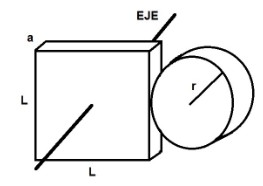
\includegraphics[width=0.4 \textwidth]{ejercicio2.jpg}
    \caption{Figura para la resolución del ejercicio 2.}
\end{figure}

\begin{justify}
    Determinar el momento de inercia de un paralelepípedo de densidad \((\rho)\)
    y de dimensiones \(( L \times L \times a )\) que tiene pegado a uno de sus lados un cilindro de radio \((r)\), altura
    \((a)\) y densidad también \((\rho)\).
\end{justify}

\begin{justify}
    El cálculo se realizará respecto a un eje que pasa por el centro del
    paralelepípedo y es perpendicular a su cara superior.
\end{justify}

\subsection{Solución.}

\textbf{Datos:}

\vspace{\baselineskip}

\textbf{Paralelepípedo}

\begin{itemize}
    \item Dimensiones \(\Rightarrow D = L \times L \times a.\)
    \item Densidad \(\Rightarrow \rho .\)
\end{itemize}

\vspace{\baselineskip}

\textbf{Cilindro.}

\begin{itemize}
    \item Radio \(\Rightarrow r.\)
    \item Altura \(\Rightarrow a.\)
\end{itemize}

\begin{justify}
    \textbf{Momentos de inercia:}
\end{justify}

\begin{multicols}{2}
    \textbf{Paralelepípedo} \( \Rightarrow I_p = \frac{1}{12}ML^2.\)
    
    \textbf{Cilindro} \(\Rightarrow I_c = \frac{1}{2}Mr^2.\)
\end{multicols}

\begin{justify}
    \textbf{Masas:}
\end{justify}

\begin{multicols}{2}
    \textbf{Paralelepípedo} \(M_p = \rho (L \times L \times a).\)

    \textbf{Cilindro} \(M_c = \rho (\pi r^2 a).\)
\end{multicols}

\begin{justify}
    Igual que en punto anterior, usaremos el \textbf{Teorema de Steiner}. Por esto, definimos la distancia \((d)\)
    entre los ejes de ambos objetos como el radio del cilindro más la mitad del ancho del paralelepípedo. 
\end{justify}

\[d = \frac{L}{2} \cdot r.\]

\newpage

\begin{justify}
    Entonces, el momento de inercia del cilindro respecto al eje de inercia del paralelepípedo es:
\end{justify}

\[I_c = \frac{1}{2} \; \rho(\pi r^2 a)r^2 + \rho \pi r^2 a \left(\frac{L}{2}+r\right)^2.\]

\begin{justify}
    El momento de inercia total es la suma de los momentos de los objetos, por esto, tenemos:
\end{justify}

\[I_{total} = \frac{1}{12} \; 2 \rho L^4 a +\frac{1}{2} \; \rho (\pi r^2 a) r^2 + \rho \pi r^2 a \left(\frac{L}{2}+r\right)^2 .\]

\begin{justify}
    Operamos y factorizamos \((\rho)\) y \((a)\).
\end{justify}


\[\boxed{ I_{total} = \rho a \left(\frac{1}{6}L^4 + \frac{1}{2} \pi r^4 + \pi r^2 \left(\frac{L}{2} + r\right)^2\right).}\]

\vspace{\baselineskip}

\section{Ejercicio.}

\begin{figure}[H]
    \centering
    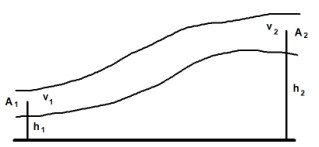
\includegraphics[width=0.5 \textwidth]{ejercicio3.jpg}
    \caption{Para la resolución del ejercicio 3.}
\end{figure}

\begin{justify}
    Por la tubería representada en la figura circula agua, de densidad \(997.13 kg/m3 \; \; (a \; 25\,^\circ\mathrm{C}).\)
\end{justify}

\begin{justify}
    Calcular, usando tanto la ecuación de continuidad como la ecuación de Bernoulli, los siguientes valores:
\end{justify}

\begin{justify}
    \textbf{Primer caso.}
\end{justify}

\begin{multicols}{2}
    \textbf{Velocidad} \(\Rightarrow v_2.\)
    
    \textbf{Área} \(\Rightarrow A_2. \)
\end{multicols}

\textbf{Con los datos:}

\begin{multicols}{4}
    \(h_1 = 4 \; m.\)
    
    \(h_2 = 10 \; m.\)

    \(A_1 = 0.125 \; m^3.\)

    \(v_1 = 10 \; m/s.\)
\end{multicols}


\begin{justify}
    \textbf{Segundo caso.}
\end{justify}

\begin{multicols}{2}
    \textbf{Velocidad} \(\Rightarrow v_1.\)
    
    \textbf{Área} \(\Rightarrow A_1. \)
\end{multicols}


\textbf{Con los datos:}


\begin{multicols}{4}
    \(h_1 = 1.5 \; m.\)
    
    \(h_2 = 2 \; m.\)

    \(A_2 = 0.025 \; m^3.\)

    \(v_2 = 1 \; m/s.\)
\end{multicols}




\subsection{Solución.}

\vspace{\baselineskip}

\subsection{Primer caso.}

\begin{justify}
    Usaremos la \textbf{Ecuación de Bernoulli.}
\end{justify}

\[P_1 + \frac{1}{2} \rho v^2_1 + \rho g h_1 = P_2 + \frac{1}{2} \rho v^2_2 + \rho g h_2\]

\vspace{\baselineskip}

\begin{justify}
    Asumiendo la presión atmosférica igual en ambas presiones:
\end{justify}

\[\frac{1}{2}v^2_1 + gh_1 = \frac{1}{2}v^2_2 + g h_2.\]

\begin{justify}
    Despejamos \(v^2\):
\end{justify}

\[v^2_2 = \frac{\frac{1}{2} v^2_1 + g h_1 - g h_2 }{\frac{1}{2}} \Rightarrow v_2 = \sqrt{2 \left(\frac{1}{2} v^2_1 + g \left(h_1 - h_2\right)\right)} \]

\vspace{\baselineskip}

\[v^2 = \sqrt{ v^2_1 + 2g\left(h_1 - h_2\right) } \Rightarrow v^2 = \sqrt{ 10^2 + 2 \cdot 9.81 \left(4 - 10\right) }\]

\[\boxed{v_2 = \sqrt{-17.72} \; m/s.}\]


\begin{justify}
    Con el resultado más la \textbf{ecuación de continuidad} podriamos obtener \((A_1)\), como hemos obtenido una raíz cuadrada negativa que no posee 
    sentido físico, optaremos por dejar el desarrollo hasta este punto.
\end{justify}

\subsection{Segundo caso.}

\begin{justify}
    Procedemos igual que el primer punto a desarrollar, hasta llegar a la expresión:
\end{justify}

\[v_1 = \sqrt{v^2_2 + 2g\left(h_2 - h_1\right)}.\]

\newpage


\begin{justify}
    Sustituyendo por nuestro datos tenemos:
\end{justify}

\[v_1 = \sqrt{1^2 + 2 \cdot 9.81 \left(2 - 1.5\right)} \Rightarrow \sqrt{10.81}. \]

\[\boxed{v_1 = 3.28 \; m/s.}\]

\begin{justify}
    Usaremos la \textbf{ecuación de continuidad} que expresa la conservación de la masa y establece que el producto del área por la velocidad 
    en cualquier sección a lo largo del flujo va a ser constante.
\end{justify}

\[A_1v_1 = A_2v_2.\]

\begin{justify}
    Sabiendo esto, y con los datos obtenidos, despejaremos \((A_1)\):
\end{justify}

\[A_1 = \frac{0.025 \; m^{\; \cancel{3}} \cdot 1 \; \cancel{m/s}}{3.28 \; \cancel{m/s}}.\]

\vspace{\baselineskip}

\[\boxed{ A_1 = 0.007621 \; m^2.}\]


\section{Ejercicio.}

\vspace{\baselineskip}

\begin{justify}
    Determinar cuáles  objetos flotarán :
\end{justify}

\begin{itemize}
    \item \textbf{Caja metálica.}
    \begin{multicols}{2}
        \(m = 3000 \; kg.\)

        \(V = 1250 \; L.\)
    \end{multicols}
    \item \textbf{Caja de madera.}
    \begin{multicols}{2}
        \(m = 200 \; kg.\)

        \(V = 50 \; L.\)
    \end{multicols}
    \item \textbf{Bola maciza.}
    \begin{multicols}{3}
        \(m = 650 \; kg.\)

        \(r = 1 \; m.\)

        \(V = \frac{4}{3} \pi r^3. \)
    \end{multicols}
\end{itemize}

\begin{justify}
    Teniendo en cuenta que la densidad del agua es \(\rho = 997.13 \; kg/m^3\) (a \(25^\circ C\)).
\end{justify}


\newpage 

\subsection{Solución.}


\begin{justify}
    El objeto flotará si el empuje es mayor o igual a su peso \((P)\), donde este es el producto de la masa por la gravedad \((m \cdot g)\).
\end{justify}

\begin{justify}
    El empuje lo encontraremos usando el \textbf{principio de Arquímedes}.
\end{justify}

\[E = \rho V g.\]

\begin{enumerate}
    \item \textbf{Caja metálica:}
    
        \(P = 3000kg \cdot 9.81m/s^2 \Rightarrow \boxed{P = 29.430 \; N.}\)
    
        \(E =  997.13 \; kg/m^3\cdot 1.25m^3 \cdot 9.81 m/s^2. \Rightarrow \boxed{E =12.227 \; N.}\)

    \item \textbf{Caja de madera: }
    
        \(P = 200kg \cdot 9.81m/s^2 \Rightarrow \boxed{P = 1.962 \;N.}\)

        \(E = 997.13 \; kg/m^3\cdot 0.05 m^3 \cdot 9.81 m/s^2. \Rightarrow \boxed{E = 489.09 \; N. }\)

    \item \textbf{Bola maciza:}
    
        \(P = 650kg \cdot 9.81 m/s^2 \Rightarrow \boxed{P = 6.376.5 \; N.}\)

        \(E = 997.13 \; kg/m^3\cdot \frac{4}{3} \pi 1^3 \cdot 9.81 m/s^2 \Rightarrow \boxed{E = 40.974 \; N. } \)
\end{enumerate}

\vspace{\baselineskip}

\begin{justify}
    Hemos dicho que para que un cuerpo flote se tiene que cumplir que \((E \geq P)\) por esto definimos:
\end{justify}

\begin{itemize}
    \item \textbf{Caja metálica} \((E < P)\) por lo tanto podemos afirmar que la caja metálica \textbf{no flotará}.
    \item \textbf{Caja de madera} \((E < P)\)  aunque la madera es un material comunmente flotable, es ta vez \textbf{no flotará}.
    \item \textbf{Bola maciza} \((E > P)\) aunque hablamos de una bola maciza, esta cumple con la ecuación, por lo tanto, \textbf{flotará}.
\end{itemize}


\vspace{\baselineskip}

\section{Calificación/Obervaciones.}

\begin{figure}[H]
    \centering
    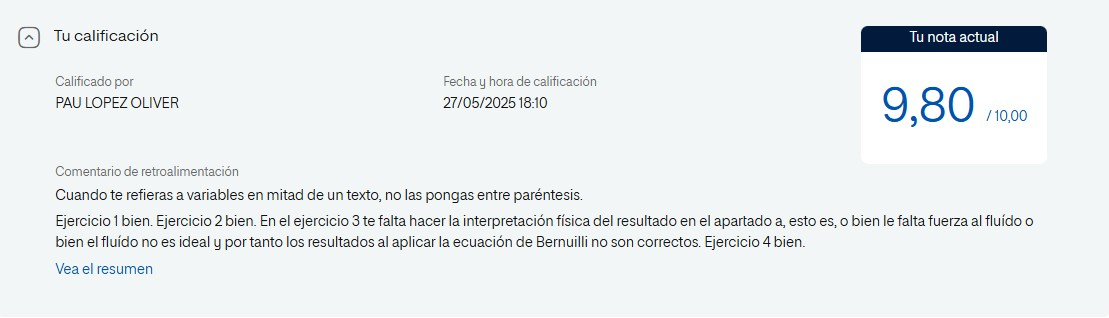
\includegraphics[width=1 \textwidth]{calificacion.jpg}
\end{figure}

\end{document}



